\documentclass{article}
\usepackage[utf8]{inputenc}
\usepackage[francais]{babel}
\usepackage[T1]{fontenc}
\usepackage{algorithmeUTF8}
\usepackage{hyperref}
\usepackage{listings}
\usepackage{graphicx}

\title{Compresseur de Huffman}
\author{Octave Queffelec \and Quentin Robcis \and Mathieu Vandecasteele \and Jean-Gabriel Wacyk \and Regis Maskembe}

\begin{document}

\pagenumbering{gobble}
\maketitle
\newpage


\tableofcontents
\newpage

\pagenumbering{arabic}

\section{Introduction}
\chapter{Introduction}

Ce rapport fait l'état de notre projet de compresseur d'Huffman en  C, dans le cadre de l'EC Algorithmique et programmation avancée dispensé en ASI3.
Le projet s'est d\'{e}roul\'{e} pendant la deuxieme moiti\'{e} du semestre 3.1.\\

L'objectif est de développer dans le language C un compresseur de type Huffman qui permet à la fois de compresser et de décompresser des fichiers.\\

Pour la r\'{e}alisation de ce projet il fallait respecter les m\'{e}thodes de programmation vues en cours, de travailler en \'{e}quipe et de r\'{e}pondre aux besoins du cahier des charges. Tout cela pour simuler au mieux possible un projet en milieu professionnel.  \\

\newpage
\section{Analyse}
\subsection{TAD}

\subsubsection{TAD codeBinaire}
\begin{tad}
  \tadNom{codeBinaire}
  \tadDependances{Bit, Booleen, Naturel}
  \begin{tadOperations}{codeBinaire}
    \tadOperation{codeBinaire}{}{\tadUnParam{codeBinaire}}
  \end{tadOperations}
\end{tad}


\subsubsection{TAD octet}
\begin{tad}
  \tadNom{octet}
  \tadDependances{Bit, Booleen, Naturel}
  \begin{tadOperations}{octet}
    \tadOperation{octet}{}{\tadUnParam{octet}}
    \tadOperationAvecPreconditions{obetnirIemeBit}{\tadDeuxParams{octet}{Naturel}}{\tadUnParam{Bit}}
    \tadOperation{completerOctet}{\tadDeuxParams{octet}{Bit}}{\tadUnParam{octet}}
    \tadOperation{estCompletOctet}{\tadUnParam{octet}}{\tadUnParam{Booleen}}
  \end{tadOperations}
  \begin{tadPreconditions}{codeBinaire}
    \tadPrecondition{obtenirIemeBit(octet)}{i>0 \& i<longueurCodeBinaire(octet)}
  \end{tadPreconditions}
\end{tad}


\subsubsection{TAD statistiques}
\begin{tad}

\tadNom{Statistiques}
\tadParametres{Element,Naturel}
\tadDependances{\booleen, Liste}

\begin{tadOperations}{Statistiques}
	\tadOperation{statistiques}{}{\tadUnParam{Statistiques}}
	\tadOperation{ajouterElement}{\tadTroisParams{Statistiques}{Element}{Naturel}}{\tadUnParam{Statistiques}}
	\tadOperationAvecPreconditions{retirerElement}{\tadDeuxParams{Statistiques}{Element}}{\tadUnParam{Statistiques}}
	\tadOperation{estPresentElement}{\tadDeuxParams{Statistiques}{Element}}{\tadUnParam{\booleen}}
	\tadOperationAvecPreconditions{obtenirValeur}{\tadDeuxParams{Statistiques}{Element}}{\tadUnParam{Naturel}}
	\tadOperation{obtenirElements}{\tadUnParam{Statistiques}}{\tadUnParam{Liste<Element>}}
	\tadOperation{obtenirValeurs}{\tadUnParam{Statistiques}}{\tadUnParam{Liste<Naturel>}}
\end{tadOperations}

\begin{tadPreconditions}{Statistiques}
	\tadPrecondition{retirerElement(stat,e)}{estPresentElement(stat,e)}	
	\tadPrecondition{obtenirValeur(stat,e)}{estPresentElement(stat,e)}
\end{tadPreconditions}

\begin{tadAxiomes}{Statistiques}
	\tadAxiome{obtenirValeur(ajouterElement(stat,e,1))=1}
	\tadAxiome{non(EstPresent(retirer(stat,e),e))}
	\tadAxiome{retirerElement(ajouterElement(stat,e,1),e)=stat}
\end{tadAxiomes}

\end{tad}

\subsubsection{TAD arbreDeHuffman}
\begin{tad}
	  \tadNom{ArbreDeHuffman}
	  \tadParametres{Élément}
	  \tadDependances{\booleen}
	  
	  \begin{tadOperations}{ArbreDeHuffman}
	    \tadOperation{arbreDeHuffman}{}{\tadUnParam{ArbreDeHuffman}}
	    \tadOperation{ajouterElement}{\tadDeuxParams{ArbreDeHuffman}{Élément}}{\tadUnParam{ArbreDeHuffman}}
	    \tadOperation{estUneFeuille}{\tadUnParam{ArbreDeHuffman}}{\tadUnParam{\booleen}}
	    \tadOperationAvecPreconditions{obtenirFilsGauche}{\tadUnParam{ArbreDeHuffman}}{\tadUnParam{ArbreDeHuffman}}
	    \tadOperationAvecPreconditions{obtenirFilsDroit}{\tadUnParam{ArbreDeHuffman}}{\tadUnParam{ArbreDeHuffman}}
	    \tadOperation{obtenirElement}{\tadUnParam{ArbreDeHuffman}}{\tadUnParam{Élément}}
	    \tadOperation{comparerElements}{\tadDeuxParams{ArbreDeHuffman}{ArbreDeHuffman}}{\tadUnParam{ArbreDeHuffman}}
            \tadOperationAvecPreconditions{fusionnerArbres}{\tadTroisParams{ArbreDeHuffman}{ArbreDeHuffman}{ArbreDeHuffman}}{\tadUnParam{ArbreDeHuffman}}
	  \end{tadOperations}
	  
	  \begin{tadPreconditions}{ArbreDeHuffman}
	  \tadPrecondition{ajouterRacine(racine,filsG,filsD)}{estUneFeuille(racine)}	
	  \tadPrecondition{obtenirFilsGauche(racine)}{non(estUneFeuille(racine))}
	  \tadPrecondition{obtenirFilsDroit(racine)}{non(estUneFeuille(racine))}
	  \end{tadPreconditions}

	  \begin{tadAxiomes}
	    \tadAxiome{estUneFeuille(arbreDeHuffman)}
	    \tadAxiome{non estUneFeuille(arbre(racine,filsG,filsD)}
	    \tadAxiome{obtenirElement(ajouterElement(racine,élément)) = Élément}
	    \tadAxiome{obtenirFilsGauche(arbre(racine,filsG,filsD)) = filsG}
	    \tadAxiome{obtenirFilsDroit(arbre(racine,filsG,filsD)) = filsD}
	    \tadAxiome{obtenirElement(arbre(racine,filsG,filsD)) = obtenirElement(filsG) + obtenirElement(filsD)}
	  \end{tadAxiomes}

\end{tad}


\subsubsection{TAD fileDePriorité d'ArbresdeHuffman}
\begin{tad}
  \tadNom{FileDePriorité}
  \tadDependances{Booleen, ArbreDeHuffman}
  \begin{tadOperations}{FileDePriorité}
    \tadOperation{file}{}{\tadUnParam{FileDePriorité}}
    \tadOperation{estVide}{\tadUnParam{FileDePriorité}}{\tadUnParam{Booleen}}
    \tadOperationAvecPreconditions{défiler}{\tadUnParam{FileDePriorité}}{\tadUnParam{FileDePriorité}}
    \tadOperationAvecPreconditions{obtenirElement}{\tadUnParam{FileDePriorité}}{\tadUnParam{ArbreDeHuffman}}
    \tadOperation{insérer}{\tadDeuxParam{FileDePriorité}{ArbreDeHuffman}}{\tadUnParam{fileDePriorité}}
  \end{tadOperations}
  \begin{tadAxiomes}
    \tadAxiome{estVide(file())}
    \tadAxiome{non estVide(insérer(file(),e))}
    \tadAxiome{défiler(insérer(file(),e))=file()}
    \tadAxiome{obtenirElément(insérer(file(),e))=e}
    \tadAxiome{non(estVide(file())) et obtenirElément(insérer(file(),e)=obtenirElément(file())}
  \end{tadAxiomes}
  \begin{tadPreconditions}{FileDePriorité}
    \tadPrecondition{défiler(f)}{non(estVide(f))}
    \tadPrecondition{obtenirElément(f)}{non(estVide(f))}
  \end{tadPreconditions}
\end{tad}


\subsubsection{TAD tableDeCodage}
\begin{tad}
  \tadNom{TableDeCodage}
  \tadDependances{Octet, CodeBinaire}

  \begin{tadOperations}{TableDeCodage}
   \tadOperation{tableDeCodage}{}{\tadUnParam{TableDeCodage}}
    \tadOperation{ajouter}{\tadDeuxParams{TableDeCodage}{CodeBinaire}}{\tadUnParam{TableDeCodage}}
    \tadOperation{estPresentCodeBinaire}{{\tadDeuxParams{TableDeCodage}{CodeBinaire}}{\tadUnParam{\Booleen}}
    \tadOperation{ObtenirCodeBinaire}{{\tadDeuxParams{TableDeCodage}{Octet}}{\tadUnParam{CodeBinaire}}
}

  \begin{tadAxiomes}{TableDeCodage}
  \tadAxiome{estPresentCodeBinaire(ajouter(tdc,cb))}
  \end{tadAxiomes}

\end{tad}



\newpage
\section{Conception}
\subsection{Analyse descendante}
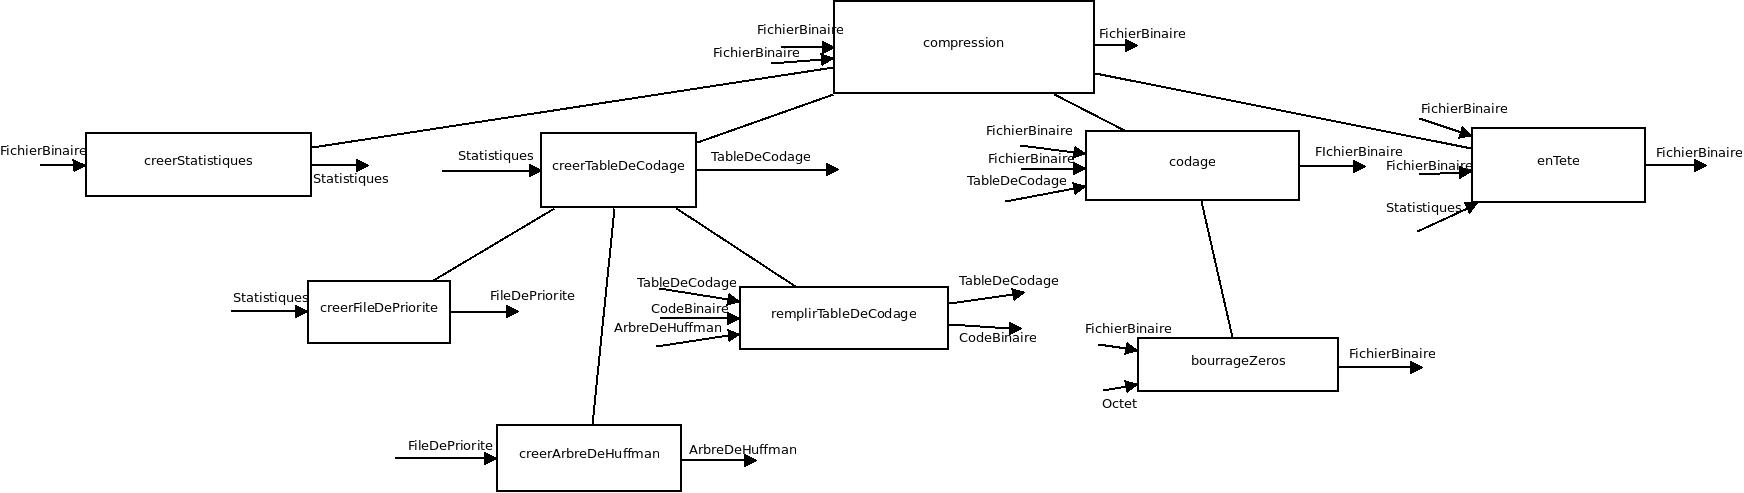
\includegraphics[width=500pt,angle=90, origin=c]{./input/Compression_Analysedescendante.jpeg}
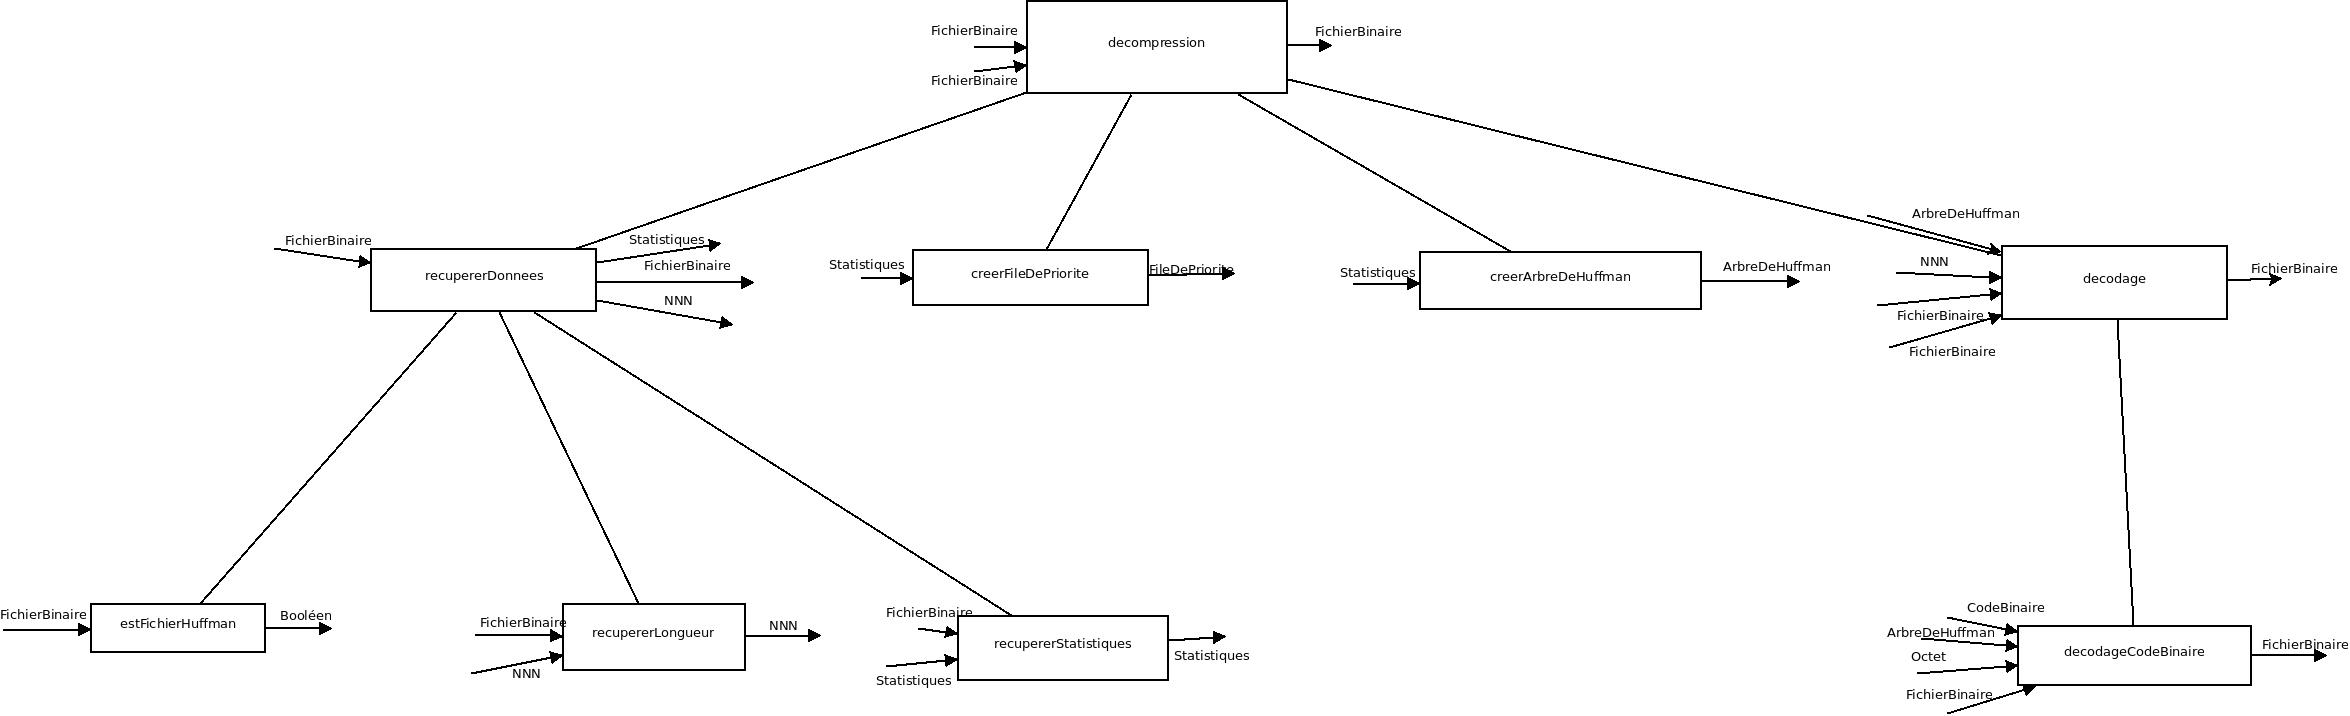
\includegraphics[width=500pt,angle=90, origin=c]{./input/decompression_analyse.jpeg}
\subsection{Conception Préliminaire}

\subsubsection{Signatures TAD arbreDeHuffman}
\begin{algolist}{0cm}
  \type{ArbreDeHuffman}{ADH\_Noeud}
%%\signatureFonctionAvecPreconditions{nom_fonction}{paramètres}{sortie}{précondition}
%%\signatureFonction{nom_fonction}{paramètres}{sortie}
  \signatureFonction{creerArbreDeHuffman}{unsigned int ponderation, char caractere}{ArbreDeHuffman}
  \signatureFonction{estUneFeuille}{ArbreDeHuffman arbre}{Booleen}
  \signatureFonctionAvecPreconditions{obtenirFilsGauche}{ArbreDeHuffman arbre}{ArbreDeHuffman}{non(estUneFeuille(arbre))}
  \signatureFonctionAvecPreconditions{obtenirFilsDroit}{ArbreDeHuffman arbre}{ArbreDeHuffman}{non(estUneFeuille(arbre))}
  \signatureFonction{obtenirPonderation}{ArbreDeHuffman arbre}{unsigned int}
  \signatureFonctionAvecPreconditions{obtenirCaractere}{ArbreDeHuffman feuille}{char}{estUneFeuille(feuille)}
  \signatureFonction{ajouterRacine}{ArbreDeHuffman arbre1, ArbreDeHuffman arbre2}{ArbreDeHuffman}
\end{algolist}


\subsubsection{Signatures TAD octet}
% auteur : Mathieu Vandecasteele
\begin{algolist}{0cm}
  \begin{enregistrement}{Octet}
    \item octet : \naturel
    \item nb : \naturel
  \end{enregistrement}

\signatureFonction{O\_getOctet}{o : Octet}{Caractere}
\\

\signatureFonction{O\_octetZero}{}{Octet}
\\

\signatureFonction{O\_nombreBit}{octet : Octet}{Entier}
\\

\signatureFonction{O\_estRempli}{o : Octet}{\booleen}
\\

\signatureFonctionAvecPreconditions{O\_obtenirBit}{o : Octet, pos : \naturel}{Bit}

\signatureProcedure{O\_ajouterPoidsFaible}{
\paramEntree bit : Bit,
\paramEntreeSortie o : Octet
}
\\

\signatureProcedure{O\_ajouterPoidsFort}{
\paramEntree bit : Bit,
\paramEntreeSortie o : Octet
}
\\

\signatureFonction{O\_octetEnDecimal}{o : Octet}{Entier}
\\

\signatureFonction{O\_decimalEnOctet}{decimal : Entier}{Octet}
\\

\signatureFonction{O\_comparerOctet}{octet1 : Octet, octet2 : Octet}{\booleen}
\\

\signatureFonction{O\_octetEnCodeBinaire}{o : Octet}{CodeBinaire}
\\

\signatureFonction{O\_codeBinaireEnOctet}{code : CodeBinaire}{Octet}

\end{algolist}


\subsubsection{Signatures TAD statistiques}
% auteur : Mathieu Vandecasteele	
\begin{algolist}{0cm}
\type{Statistiques}
\\

\signatureFonction{STAT\_statistiques}{}{Statistiques}
\\

\signatureProcedure{STAT\_ajouter}{
\paramEntree octet : Octet,
\paramEntreeSortie stats : Statistiques
}
\\

\signatureFonction{STAT\_estPresentOctet}{stats : Statistiques, octet : Octet}{\booleen}
\\

\signaturefonctionAvecPreconditions{STAT\_obtenirPonderation}{stats : Statistiques, octet : Octet}{\naturel}

\end{algolist}


\subsubsection{Signatures TAD codeBinaire}
% auteur : Mathieu Vandecasteele	
\begin{algolist}{0cm}

\type{CodeBinaire}{CB\_Noeud}
\\

\signaturefonction{CB\_codeBinaire}{CodeBinaire}
\\

\signatureprocedure{CB\_ajouter}{
\ParamEntree bit : Bit,
\ParamEntreeSortie cb : CodeBinaire
}
\\

\signaturefonction{CB\_obtenirBit}{code : CodeBinaire, position : \naturel}{Bit}
\\


\signatureprocedure{CB\_supprimerTete}{
\ParamEntreeSortie code : CodeBinaire
}
\\


\signatureprocedure{CB\_supprimer}{
\ParamEntreeSortie code : CodeBinaire
}
\\

\signaturefonction{CB\_longueur}{code : CodeBinaire}{\naturel}
\\

\signaturefonction{CB\_copie}{code : CodeBinaire}{CodeBinaire}
\\

\signaturefonction{CB\_compareCodeBinaire}{code1 : CodeBinaire, code2 :CodeBinaire}{\booleen}

\end{algolist}


\subsubsection{Signatures TAD fileDePriorité}
% auteur : Mathieu Vandecasteele	
\begin{algolist}{0cm}

\type{FileDePriorite}{FDP\_Noeud}
\\

\signatureprocedure{FDP\_ajouter}{
\ParamEntree stats : Statistiques,
\ParamEntreeSortie fdp : FileDePriorite
}
\\

\signaturefonction{STAT\_obtenirFileSuivante}{file : FileDePriorite}{FileDePriorite}
\\

\signatureprocedure{FDP\_fixerListeSuivante}{
\ParamEntree file : FileDePriorite,
\ParamEntreeSortie fileReceveuse : FileDePriorite
}
\\

\signaturefonction{FDP\_fileDePriorite}{FileDePriorite}
\\

\signaturefonction{FDP\_estVide}{file : FileDePriorite}{\booleen}
\\

\signatureprocedure{FDP\_enfilerADH}{
\ParamEntree arbre : ArbreDeHuffman,
\ParamEntreeSortie file : FileDePriorite
}
\\

\signaturefonction{FDP\_obtenirADH}{file : FileDePriorite}{ArbreDeHuffman}
\\

\signaturefonction{FDP\_longueur}{file : FileDePriorite}{\naturelNonNul}
\\

\signatureprocedure{FDP\_defilerADH}{
\ParamEntreeSortie file : FileDepriorite
}

\end{algolist}


\subsubsection{signatures TAD tableDeCodage}
% auteur : Mathieu Vandecasteele	
\begin{algolist}{0cm}

\type{TableDeCodage}
\\

\signaturefonction{TDC\_tableDeCodage}{TableDeCodage}
\\

\signatureprocedure{TDC\_ajouter}{
\ParamEntree o : Octet, cb : CodeBinaire,
\ParamEntreeSortie tdc : TableDeCodage
}
\\

\signaturefonction{TDC\_estPresentCodeBinaire}{tdc : TableDeCodage, o : Octet, cb : CodeBinaire}{\booleen}
\\

\signaturefonction{TDC\_obtenirCodeBinaire}{tdc : TableDeCodage, o : Octet}{CodeBinaire}

\end{algolist}


\subsubsection{Signatures compression}
%auteur : Mathieu Vandecasteele

\begin{algolist}

% procedure compression(E fichierSource : FichierBinaire, E/S fichierDestination : FichierBinaire)
\signatureprocedure{compression}{
		\paramEntree  fichierSource : FichierBinaire,
		\paramEntreeSortie fichierDestination : FichierBinaire
}
\\

% fonction creerStatistiques(fichier : FichierBinaire) : Statistiques
\signatureFonction{creerStatistiques}{fichier : FichierBinaire}{Statistiques}
\\

% fonction creerTableDeCodage(stats : Statistiques) : TableDeCodage
\signatureFonction{creerTableDeCodage}{stats : Statistiques}{TableDeCodage}
\\

% procedure codage(E fichierSource : FichierBinaire, tdc : TableDeCodage, E/S fichierDestination : FichierBinaire)
\signatureprocedure{codage}{
  \paramEntree fichierSource : FichierBinaire, tdc : TableDeCodage,
  \paramEntreeSortie fichierDestination : FichierBinaire
  }
\\

% procedure enTete(E fichierSource : FichierBinaire, stats : Statistiques, E/S fichierDestination : FichierBinaire)
\signatureprocedure{enTete}{
  \paramEntree fichierSource : FichierBinaire, stats : Statistiques,
  \paramEntreeSortie fichierDestination : FichierBinaire
  }
\\

% fonction creerFileDePriorite(stats : Statistiques) : FileDePriorite
\signatureFonction{creerFileDePriorite}{stats : Statistiques}{FileDePriorite}
\\

% procedure remplirTableDeCodage(E/S tdc : TableDeCodage, code : CodeBinaire, arbre : ArbreDeHuffman)
\signatureprocedure{remplirTableDeCodage}{
    \paramEntreeSortie tdc : TableDeCodage, code : CodeBinaire, arbre : ArbreDeHuffman
  }
\\

% procedure bourrageZeros(E/S fichier : FichierBinaire, E octetAEcrire : Octet)
\signatureProcedure{bourrageZeros}{
	\paramEntreeSortie fichier : FichierBinaire,
	\paramEntree octetAEcrire : Octet
}

\\

% fonction creerArbreDeHuffman(file : FileDePriorite) : ArbreDeHuffman
\signatureFonction{creerArbreDeHuffman}{file : FileDePriorite}{ArbreDeHuffman}

\end{algolist}



\subsubsection{Signatures décompression}
% auteur : Mathieu Vandecasteele

\begin{signaturesdecompression}

% procedure decompression(E fichierSource : FichierBinaire, E/S fichierDestination : FichierBinaire)
\signatureprocedure{decompression}{
		\paramEntree  fichierSource : FichierBinaire,
		\paramEntreeSortie fichierDestination : FichierBinaire
}
\\

% procedure recupererDonnees(E/S fichierSource : FichierBinaire, S stats : Statistiques, longueur : NaturelNonNul)
\signatureProcedure{recupererDonnees}{
	\paramEntreeSortie fichierSource : FichierBinaire,
	\paramSortie stats : Statistiques, longueur : \naturelNonNul
}
\\

% fonction creerFileDePriorite(stats : Statistiques) : FileDePriorite
\signatureFonction{creerFileDePriorite}{stats : Statistiques}{FileDePriorite}
\\

% fonction creerArbreDeHuffman(file : FileDePriorite) : ArbreDeHuffman
\signatureFonction{creerArbreDeHuffman}{file : FileDePriorite}{ArbreDeHuffman}
\\

% procedure decodage(E fichierSource : FichierBinaire, longueur : NaturelNonNul, adh : ArbreDeHuffman, E/S fichierDest : FichierBinaire)
\signatureProcedure{decodage}{
		\paramEntree  fichierSource : FichierBinaire, longueur : \naturelNonNul, adh : ArbreDeHuffman,
		\paramEntreeSortie fichierDest : FichierBinaire
}
\\

% fonction estFichierHuffman(fichier : FichierBinaire) : Booléen
\signatureFonction{estFichierHuffman}{fichier : FichierBinaire}{\booleen}
\\

% procedure recupererLongueur(E fichierSource : FichierBinaire, E/S longueur : NaturelNonNul)
\signatureProcedure{recupererLongueur}{
	\paramEntree fichierSource : FichierBinaire,
	\paramEntreeSortie longueur : \naturelNonNul
}
\\

% procedure recupererStatistiques(E fichierSource : FichierBinaire, E/S stats : Statistiques)
\signatureProcedure{recupererStatistiques}{
	\paramEntree fichierSource : FichierBinaire,
	\paramEntreeSortie stats : Statistiques
}
\\

% procedure decodageCodeBinaire(E cbACoder : CodeBinaire, adh : ArbreDeHuffman, S octet : Octet, trouve : Booleen)
\signatureprocedure{decodageCodeBinaire}{
		\paramEntree  cbACoder : CodeBinaire, adh: ArbreDeHuffman,
		\paramSortie octet : Octet, trouve : \booleen
}

\end{signaturesdecompression}


 \subsection{Conception Détaillée}

 \subsubsection{Codage}
 % auteur : Wacyk Jean-Gabriel

\begin{algorithme}
  \procedure{bourrageZeros}{
  \paramEntree{octetAecrire : Octet}
  \paramEntreeSortie{dest : FichierBinaire}
  }
  {}
  {
  \sialors{non(nombreBit(octetAecrire)=0)}
      {
      \tantque{nombreBit(octetAecrire)<8}
        {
        \instruction{ajouterPoidsFort(octetAecrire,bitA0)}
        }
      \instruction{ecrireOctet(dest)}
      }
  }
\end{algorithme}

\begin{algorithme}
  \procedure{codage}{
  \paramEntree{source : FichierBinaire, tdc :TableDeCodage}
  \paramEntreeSortie{dest : FichierBinaire}
  }
  {
  octetAecrire : Octet\\
  octetAlire : Octet\\
  code : CodeBinaire\\
  i : \naturel
  }
  {
  \affecter{octetAecrire}{octetZero()}
  \affecter{octetAlire}{octetZero()}
  \instruction{deplacerCurseur(source,0)}
  \tantque{lireOctet(source,octetAlire)=1 et finfichier(source)=0}
  {
    \affecter{code}{codeBinaire()}
    \pour{i}{0}{longueur(code)}{}
      {
      \instruction{ajouterPoidsFort(octetAecrire,obtenirBit(code,i+1))}
      \sialors{estRemplis(octetAecrire)}
        {
        \instruction{ecrireOctet(dest,octetAecrire)}
        \affecter{octetAecrire}{octetZero()}
        }
      }
    }
    \instruction{bourrageZeros(dest,octetAecrire)}
  }
\end{algorithme}


 \subsubsection{Compression}
 % auteur : Mathieu Vandecasteele
\begin{algorithme}
	\procedure{compression}{
		\paramEntree  fichierSource : FichierBinaire
		\paramSortie fichierDestination : FichierBinaire
	}{
		stat : Statistiques
		tdc: TableDeCodage
		
	}{
		\affecter{stat}{creerStatistiques(fichierSource)}
		\affecter{tdc}{creerTableDeCodage(stat)}
		\instruction{enTete(FichierSource,FichierDestination,stat)}
		\instruction{codage(FichierSource,FichierDestination,tdc)}

	}
\end{algorithme}


 \subsubsection{creerFileDePriorité}
 % auteur : Wacyk Jean-Gabriel

\begin{algorithme}
  \fonction{creerFileDePriorite}{stat : Statistiques}{FileDePriorite}
  {
    file : FileDePriorite \\
    feuille : ArbreDeHuffman
	}
  {
    \affecter{file}{fileDePriorite()}
    \pour{i}{0}{STATSIZE}{}
      {
      \sialors{estPresentOctet(stat,decimalEnOctet(i))}
        {
        \affecter{feuille}{arbreDeHuffman(obtenirPonderation(stat,decimalEnOctet(i)),decimalEnOctet(i))}
        {insérer(file,feuille)}
        }
      }
  \retourner{file}
  }
\end{algorithme}


 \subsubsection{creerStatistiques}
 % auteur : Wacyk Jean-Gabriel

\begin{algorithme}
  \fonction{creerStatistiques}{fichier : FichierBinaire}{Statistiques}
  {
  stat : Statistiques \\
  octet : Octet
	}
  {
  \affecter{octet}{octet()}
  \affecter{stat}{statistiques()}
  \tantque{lireOctet(fichier,octet)=1 ET finfichier(fichier)=0}{
  {ajouter(stat,octet)}
  }
  \retourner{stat}
  }
\end{algorithme}


 \subsubsection{creerTableDeCodage}
 % auteur : Wacyk Jean-Gabriel

\begin{algorithme}
  \fonction{creerArbreDeHuffman}{file : FileDePriorite}{ArbreDeHuffman}
  {
  temp : ArbreDeHuffman\\
  arbre1 : ArbreDeHuffman\\
  arbre2 : ArbreDeHuffman
  }
  {
  \tantque{non(longueur(file)=1)}
    {
    \affecter{arbre1}{obtenirElement(file)}
    \instruction{défiler(file)}
    \affecter{arbre2}{obtenirElement(file)}
    \instruction{défiler(file)}
    \affecter{temp}{ajouterRacine(arbre1,arbre2)}
    \instruction{insérer(file,temp)}
    }
  \retourner{temp}
  }\\
\end{algorithme}

\begin{algorithme}
  \procedure{remplirTableDeCodage}{
    \paramEntreeSortie{tdc : TableDeCodage, arbre : ArbreDeHuffman, code : CodeBinaire}
  }
  {
  temp : CodeBinaire
  }
  {
  \sialorssinon{estUneFeuille(arbre)}
  {
    \affecter{temp}{copie(code)}
    \instruction{ajouter(tdc,obtenirCaractere(arbre),temp)}
    \instruction{supprimerTete(code)}
  }
  {
    \instruction{ajouter(code,bitA0)}
    \instruction{ramplirTableDeCodage(tdc,obtenirFilsGauche(arbre),code)}
    \instruction{ajouter(code,bitA1)}
    \instruction{ramplirTableDeCodage(tdc,obtenirFilsDroit(arbre),code)}
    \sialors{non(longueur(code)=0)}
      {
      \instruction{supprimerTete(code)}
      }
  }
  }\\
\end{algorithme}

\begin{algorithme}
  \fonction{creerTableDeCodage}{stats : Statistiques}{TableDeCodage}
  {
  code : CodeBinaire\\
  res : TableDeCodage\\
  arbre : ArbreDeHuffman\\
  file : FileDePriorite
  }
  {
  \affecter{code}{codeBinaire()}
  \affecter{res}{tableDeCodage()}
  \affecter{file}{creerFileDePriorite(stats)}
  \affecter{arbre}{creerArbreDeHuffman(file)}
  \instruction{remplirTableDeCodage(res,arbre,code)}
  \retourner{res}
  }
\end{algorithme}


 \subsubsection{decodage}
 % auteur : Octave Queffelec
\begin{algorithme}
	\procedure{decodage}{
		\paramEntree  fichierSource : FichierBinaire, longueur: \naturel, adh : ArbreDeHuffman
		\paramEntreeSortie fichierDest : FichierBinaire
	}{
		posCurseur : \naturel
		i : \naturel
		octetAlire : Octet\\
		octetAecrire : Octet\\
		cbAdecoder : CodeBinaire\\
		cbAdecoderInverse : CodeBinaire

	}{
		\affecter{posCurseur}{0}
		\affecter{octetAlire}{octetZero()}
		\affecter{octetAecrire}{octetZero()}
		\affecter{cbAdecoder}{codeBinaire()}
		\affecter{cbAdecoderInverse}{codeBinaire()}

		\tantque{(posCurseur <= longeur-1) et (non(finFichier(fichierSource)))  et (lireOctet(fichierSource,octetAlire))}{
			\affecter{trouve}{FAUX}
			\affecter{i}{0}
			\tantque{(i<8) et (posCurseur<longueur-1)}{
				\instruction{ajouter(cbAdecoder,\instruction{obtenirBit(octetAlire,7-i)}}
				\affecter{cbAdecoderInverse}{\instruction{copie(cbAdecoder)}}
				\instruction{decodageCodeBinaire(cbAdecoder,adh,octetAlire,trouve)}
				\sialors{trouve}{
					\instruction{ecrireOctet(fichierDest,octetAecrire)}
					\affecter{cbAdecoder}{codeBinaire()}
					\affecter{cbAdecoderInverse}{codeBinaire()}
					\affecter{posCurseur}{posCurseur+1}
					}
				\affecter{i}{i+1}
				}
			}
		}
\end{algorithme}


 \subsubsection{decodageCodeBinaire}
 % auteur : Octave Queffelec
\begin{algorithme}
	\procedure{decodageCodeBinaire}{
		\paramEntree  cbAcoder : CodeBinaire, adh: ArbreDeHuffman
		\paramSortie octet : Octet, trouve : \booleen
	}{
		i:\naturel
		adhTemp: ArbreDeHuffman

	}{
		\affecter{adhTemp}{adh}
		\affecter{trouve}{FAUX}
		\pour{i}{0}{longueur(cbAdecoder)}{}{
			\sialorssinon{obtenirBit(cbAdecoder,i+1)=bitA0}{
				\affecter{adhTemp}{obtenirFilsGauche(adhTemp)}
				}{
				\affecter{adhTemp}{obtenirFilsDroit(adhTemp)}
				}}
		\sialors{estUneFeuille(adhTemp)}{
			\affecter{octet}{obtenirCaractere(adhTemp)}
			\affecter{trouve}{VRAI}
			}
			}
\end{algorithme}


 \subsubsection{decompression}
 %auteur : Quentin Robcis

\begin{algorithme}
  \procedure{decompression}{
    \paramEntreeSortie{fichierSource : FB\_FichierBinaire, *fichierDest : FB\_FichierBinaire}
    }
    {
    stat : STAT\_Statistiques\\
    adh : ArbreDeHuffman\\
    fdp : FDP\_FileDePriorite\\
    longueur : Naturel
    }
    {
    \affecter{stat}{STAT\_statistiques()}
    \affecter{fdp}{FDP\_fileDePriorite()}
    \affecter{longueur}{0}
    \instruction{recupererDonnees(fichierSource, \&stat, \&longueur)}
    \affecter{fdp}{creerFileDePriorite(stat)}
    \affecter{adh}{creerArbreDeHuffman(fdp)}
    \instruction{decodage(fichierDest,fichierSource,longueur,adh)}
    \instruction{FB\_deplacerCurseur(fichierDest, 0)}
    }
\end{algorithme}


 \subsubsection{enTete}
 %auteur : Quentin Robcis

\begin{algorithme}
  \procedure{enTete}{
    \paramEntreeSortie{fichierSource : FB\_FichierBinaire, *fichierDest : FB\_FichierBinaire, stat : STAT\_Statistiques}
    }
    {
    identifiant : ChaineDeCaractere\\
    longueur, i : Naturel
    }
    {
    \affecter{identifiant}{"huffman"}
    \affecter{longueur}{FB\_longueurFichier}
    \instruction{FB\_ecrireChaine(fichierDest, identifiant)}
    \instruction{FB\_ecrireNaturel(fichierDest, longueur)}
    \pour{i}{0}{STAT\_SIZE}{}
    {
    \instruction{FB\_ecrireNaturel(fichierDest, STAT\_obtenirPonderation(stat,O\_decimalEnOctet(i)))}
    }
    }
\end{algorithme}


 \subsubsection{main}
 %auteur : Quentin Robcis

\begin{algorithme}
  \fonction{main}{argc : Naturel, *argv : ChaineDeCaractere}{Naturel}
  {
  fichierCompresse : FB\_FichierBinaire\\
  fichierOrignial : FB\_FichierBinaire\\
  nomFichier : ChaineDeCaractere
  }
  {
  \sialorssinon{(argc!=0) ou ((strcmp(argv[1],"c")!=0) et (strcmp(argv[1],"d")!=0))}
  {\instruction{printf("Veuillez respecter la syntaxe suivante : \\
  Pour compresser : huffman c nomFichier\\
  pour decompresser : huffman d nomFichier.huff")}
  }
  {
    \sialorssinon{strcmp(argv[1],"c")=0}
    {
    \instruction{printf("Compression...")}
    \instruction{strcpy(nomFichier, argv[2])}
    \instruction{strcat(nomFichier,".huff")}
    \affecter{fichierOriginal}{FB\_ouvrir(argv[2],lecture)}
    \affecter{fichierCompresse}{FB\_ouvrir(nomFichier, ecriture)}
    \instruction{compression(fichierOriginal, \&fichierOriginal)}
    \instruction{printf("terminé avec succes")}
    }
    {
    \instruction{printf("Decompression...")}
    \instruction{strcpy(nomFichier, argv[2])}
    \affecter{nomFichier[strlen(nomFichier) - strlen(".huff")]}{'\textbackslash0'}
    \affecter{fichierCompresse}{FB\_ouvrir(argv[2],lecture)}
    \affecter{fichierOriginal}{FB\_ouvrir(nomFichier,ecriture)}
    \instruction{decompression(fichierCompresse, \&fichierOriginal)}
    \instruction{printf(terminé avec succes)}
    }
  }
  \retourner{EXIT\_SUCCESS}
  }\\
\end{algorithme}


 \subsubsection{recupererDonnees}
 %auteur : Quentin Robcis

\begin{algorithme}
  \fonction{estFichierHuffman}{fichierSource : FB\_FichierBinaire}{\booleen}
  {
  huffman : ChaineDeCaracteres\\
  id : Tableau[1..8]de Caracteres\\
  }
  {
  \affecter{huffman}{"huffman"}
  \affecter{id}{FB\_lireChaine(fichierSource, 7)}
  \affecter{id[8]}{'\textbackslash0'}
  \sialorssinon{strcmp(id, huffman)=0}
  {\retourner{VRAI}}
  {\retourner{FAUX}}
  }\\
\end{algorithme}

\begin{algorithme}
  \procedure{recupererLongueur}{
    \paramEntreeSortie{fichierSource : FB\_FichierBinaire, *longueur : Naturel}
    }
    {
    }
    {
    \instruction{FB\_lireNaturel(fichierSource, longueur)}
    }\\
\end{algorithme}

\begin{algorithme}
  \procedureAvecPreconditions{recupererStatistiques}{
    \paramEntreeSortie{fichierSource : FB\_FichierBinaire, *stat : STAT\_Statistiques}
    }
    {
    estFichierHuffman(fichierSource)
    }
    {
    iStat, i, j : Naturel
    }
    {
    \affecter{iStat}{0}
    \pour{i}{0}{STAT\_SIZE}{}
      {
      \instruction{FB\_lireNaturel(fichierSource, \&iStat)}
      \pour{j}{0}{iStat}{}
        {
        \instruction{STAT\_ajouter(stat,O\_decimalEnOctet(i))}
        }
      }
    }\\
\end{algorithme}

\begin{algorithme}
  \procedure{recupererDonnees}{
    \paramEntreeSortie{fichierSource : FB\_FichierBinaire, *stat : STAT\_Statistiques, *longueur : Naturel}
    }
    {

    }
    {
    \instruction{recupererLongueur(fichierSource, longueur)}
    \instruction{recupererStatistiques(fichierSource, stat)}
    }
\end{algorithme}



\newpage
\section{Code Source}
\subsection{Code source include}

\subsubsection{TAD}
\lstinputlisting{../programme/include/ArbreDeHuffman.h}
\lstinputlisting{../programme/include/Bit.h}
\lstinputlisting{../programme/include/CodeBinaire.h}
\lstinputlisting{../programme/include/FichierBinaire.h}
\lstinputlisting{../programme/include/FileDePriorite.h}
\lstinputlisting{../programme/include/Mode.h}
\lstinputlisting{../programme/include/Octet.h}
\lstinputlisting{../programme/include/Statistiques.h}
\lstinputlisting{../programme/include/TableDeCodage.h}

\subsubsection{Fonctions métier}
\lstinputlisting{../programme/include/codage.h}
\lstinputlisting{../programme/include/compression.h}
\lstinputlisting{../programme/include/creerFileDePriorite.h}
\lstinputlisting{../programme/include/creerStatistiques.h}
\lstinputlisting{../programme/include/creerTableDeCodage.h}
\lstinputlisting{../programme/include/decodage.h}
\lstinputlisting{../programme/include/decodageCodeBinaire.h}
\lstinputlisting{../programme/include/decompression.h}
\lstinputlisting{../programme/include/enTete.h}
\lstinputlisting{../programme/include/recupererDonnees.h}

\subsection{Code source src}

\subsubsection{TAD}
\lstinputlisting{../programme/src/ArbreDeHuffman.c}
\lstinputlisting{../programme/src/CodeBinaire.c}
\lstinputlisting{../programme/src/FichierBinaire.c}
\lstinputlisting{../programme/src/FileDePriorite.c}
\lstinputlisting{../programme/src/Mode.c}
\lstinputlisting{../programme/src/Octet.c}
\lstinputlisting{../programme/src/Statistiques.c}
\lstinputlisting{../programme/src/TableDeCodage.c}

\subsubsection{Fonctions métier}
\lstinputlisting{../programme/src/codage.c}
\lstinputlisting{../programme/src/compression.c}
\lstinputlisting{../programme/src/creerFileDePriorite.c}
\lstinputlisting{../programme/src/creerStatistiques.c}
\lstinputlisting{../programme/src/creerTableDeCodage.c}
\lstinputlisting{../programme/src/decodage.c}
\lstinputlisting{../programme/src/decodageCodeBinaire.c}
\lstinputlisting{../programme/src/decompression.c}
\lstinputlisting{../programme/src/enTete.c}
\lstinputlisting{../programme/src/recupererDonnees.c}
\lstinputlisting{../programme/src/main.c}

\subsection{Code source tests}

\lstinputlisting{../programme/testsrc/testCreerFileDePriorite.c}
\lstinputlisting{../programme/testsrc/testCreerTableDeCodage.c}
\lstinputlisting{../programme/testsrc/testTADCodeBinaire.c}
\lstinputlisting{../programme/testsrc/testTADArbreDeHuffman.c}
\lstinputlisting{../programme/testsrc/testTADFileDePriorite.c}
\lstinputlisting{../programme/testsrc/testTADOctet.c}
\lstinputlisting{../programme/testsrc/testTADStatistiques.c}
\lstinputlisting{../programme/testsrc/testTADTableDeCodage.c}


\newpage
\section{Conclusion}
Le projet a \'{e}t\'{e} réussi dans l'ensemble et cloturé dans le temps qui nous etait imparti. \\

Neanmoins, nous avons eu quelques petites difficultés nottament au moment de la conception de nos TAD. Dans un premier temps, nous avons mal saisis l'utilité du TAD Octet, et avons fais fausse route en implementant un tableau contenant le type Bit. Nous avons ensuite corrigé en comprenant que la lecture et l'ecriture d'octet dans des fichiers en C se faisait avec un unsigned char.

Un autre probleme qui nous a perturbé au moment de la conception detaillé : dans les procedures de codage et decodage, nous avons voulu concatener les codebinaires pour n'en former qu'un seul qui sera ensuite ecris dans le fichier copresse, ou bien decodé puis ecris dans le fichier decompresse. Or pendant la phase de développement, nous nous sommes apercu qu'à l'execution la procedure de concatenation plantais pour des fichiers de taille superieur a 2\^{}15 octets. Nous avons donc decidé de coder et de decoder les octets un par un.

Malgr\'{e} la r\'{e}ussite du projet il y a des points que nous aurions pu am\'{e}liorer. Nottament l'implementation d'un buffer pour le type FichierBinaire. En effet, la lecture et ecriture d'octet se fait un par un dans le fichier. Le temps d'execution est donc long pour des fichiers volumineux. Pour exemple, un fichier de 10Mo est compressé en 10 secondes.

Pour finir, nous avons bien respecté la méthodologie du cours et les differentes phase explicité dans l'enonce.


\newpage
\section{Cahier de suivi}
\subsection{Suivi chronologique}

\begin{table}[h]
\centering
\begin{tabular}{|c|c|l|}
\hline
Séance                                                     & Date                                                              & Travail réalisé                                                                                                                                                  \\ \hline
1                                                          & 02/12/2016                                                        & Spécification des TAD                                                                                                                                            \\ \hline
2                                                          & 09/11/2016                                                        & \begin{tabular}[c]{@{}l@{}}Analyse descendante de compression et decompression\end{tabular}                                                    \\ \hline
3                                                          & 16/11/2016                                                        & Conception préliminaire                                                                                                                                          \\ \hline
4                                                          & 23/11/2016                                                        & Conception détaillée                                                                                                                                             \\ \hline
5                                                          & 30/11/2016                                                        & \begin{tabular}[c]{@{}l@{}}Développement des TAD\\ + leurs tests unitaires\end{tabular}                                                                          \\ \hline
6                                                          & 07/12/2016                                                        & \begin{tabular}[c]{@{}l@{}}Développement des TAD et des fonctions \\ + leurs tests unitaires\end{tabular}                                                        \\ \hline
7                                                          & 14/12/2015                                                        & Développement des fonctions et des tests unitaires                                                                                                               \\ \hline
\begin{tabular}[c]{@{}c@{}}Vacances\\ de Noël\end{tabular} & \begin{tabular}[c]{@{}c@{}}16/12/2016\\ - 03/01/2017\end{tabular} & \begin{tabular}[c]{@{}l@{}} Finalisation du développement\\ Finalisation du rapport\end{tabular} \\ \hline
\end{tabular}
\end{table}

Le rapport en \LaTeX{} était tenu à jour au fur et à mesure de l'avancement.

\subsection{Répartition des tâches}

\noindent RM : Régis MASKEMDE\\
QR : Quentin ROBCIS\\
OQ : Octave QUEFFELEC\\
MV : Mathieu VANDECASTEELE\\
JW : Jean-Gabriel WACYK\\

\begin{table}[h]
\centering
\begin{tabular}{l|c|c|c|c|c|}

\cline{2-6}
                                                        & RM & QR & OQ & MV & JW \\ \hline
\multicolumn{1}{|l|}{Analyse descendante}               & X                     & X              & X                     & X                     & X                      \\ \hline
\multicolumn{1}{|l|}{makefile}                          & X                      & X              & X                     & X                     & X                      \\ \hline
\multicolumn{1}{|l|}{Octet.h}                         &                       &                &                      &                       & X                       \\ \hline
\multicolumn{1}{|l|}{CodeBinaire.h}                            &                       &                &                      &                       & X                     \\ \hline
\multicolumn{1}{|l|}{Statistiques.h}                        &                      &                &                       & X                       &                        \\ \hline
\multicolumn{1}{|l|}{ArbreDeHuffman.h}                            &                       & X              &                       &                       &                        \\ \hline
\multicolumn{1}{|l|}{FileDePriorite.h}                           & X                       &               &                       &                       &                        \\ \hline
\multicolumn{1}{|l|}{TableDeCodage.h}                         & X                       &                &                       &                       &                        \\ \hline
\multicolumn{1}{|l|}{FichierBinaire.h}       &                      &                & X                      &                       &                        \\ \hline
\multicolumn{1}{|l|}{Mode.h}           &                       &                & X                     &                       &                        \\ \hline
\multicolumn{1}{|l|}{Bit.h}               &                       &               & X                    &                       &                        \\ \hline
\multicolumn{1}{|l|}{codage.h}            &                       &                & X                       &                       &                       \\ \hline
\multicolumn{1}{|l|}{compression.h}             &                       &                & X                      &                       &                       \\ \hline
\multicolumn{1}{|l|}{creerStatistiques.h}                  &                       &               &                       & X                       &                        \\ \hline
\multicolumn{1}{|l|}{creerFileDePriorite.h}                             &                       & X              &                       &                       &                        \\ \hline
\multicolumn{1}{|l|}{creerTableDeCodage.h}                         &                       &                &                      &                       & X                        \\ \hline
\multicolumn{1}{|l|}{decodage.h}                            &                       &                &                      &                       & X                        \\ \hline
\multicolumn{1}{|l|}{decodageCodeBinaire.h}                            &                       &                &                      &                       & X                        \\ \hline
\multicolumn{1}{|l|}{decompression.h}                            &                       &                & X                     &                       &                        \\ \hline
\multicolumn{1}{|l|}{enTete.h}                            &                       &                & X                     &                       &                        \\ \hline
\multicolumn{1}{|l|}{recupererDonnees.h}                            &                       &                & X                     &                       &                        \\ \hline
\multicolumn{1}{|l|}{ArbreDeHuffman.c}                            &                       & X                &                      &                       &                        \\ \hline
\multicolumn{1}{|l|}{FileDePriorite.c}                            & X                      &                &                      &                       &                        \\ \hline
\multicolumn{1}{|l|}{TableDeCodage.c}                        & X                     &                &                       &                       &                        \\ \hline
\multicolumn{1}{|l|}{FichierBinaire.c}                        &                      &                & X                    &                       &                        \\ \hline
\multicolumn{1}{|l|}{codage.c}                        &                      &                & X                     &                       &                        \\ \hline
\multicolumn{1}{|l|}{compression.c}                        &                      &                & X                      &                       &                        \\ \hline
\multicolumn{1}{|l|}{creerStatistiques.c}                        &                      &                &                       & X                       &                        \\ \hline
\multicolumn{1}{|l|}{creerFileDePriorite.c}                        &                     & X               &                       &                       &                        \\ \hline
\multicolumn{1}{|l|}{creerTableDeCodage.c}                        &                      &                &                       &                       & X                       \\ \hline
\multicolumn{1}{|l|}{decodage.c}                        &                      &                &                       &                       & X                       \\ \hline
\multicolumn{1}{|l|}{decodageCodeBinaire.c}                            &                       &               &                       &                       & X                      \\ \hline
\multicolumn{1}{|l|}{decompression.c}                           &                       &               & X                      &                       &                        \\ \hline
\multicolumn{1}{|l|}{enTete.c}                         &                       &                & X                     &                       &                        \\ \hline
\multicolumn{1}{|l|}{recupererDonnees.c}              &                      &                & X                      &                       &                        \\ \hline
\multicolumn{1}{|l|}{main.c}                            &                       &               & X                       &                       &                        \\ \hline
\multicolumn{1}{|l|}{testTAD(tous).c}             &                       &                & X                      &                      &                        \\ \hline
\multicolumn{1}{|l|}{testCreerStatistiques.c}          &                       &               &                       &                       & X                       \\ \hline
\multicolumn{1}{|l|}{testCreerFileDePriorite.c}       &                       &                &                       &                      & X                       \\ \hline
\multicolumn{1}{|l|}{testCreerTableDeCodage.c}           &                       &                &                       &                       & X                      \\ \hline
\multicolumn{1}{|l|}{Rapport - Intro/Conclusion}        &                       &                & X                      &                       & X                      \\ \hline
\multicolumn{1}{|l|}{Rapport - TAD}                     & X                     & X              & X                     & X                     & X                      \\ \hline
\multicolumn{1}{|l|}{Rapport - Conception Préliminaire} &                       &               &                      & X                     &                        \\ \hline
\multicolumn{1}{|l|}{Rapport - Conception détaillée}    & X                     & X              & X                     & X                     & X                      \\ \hline
\multicolumn{1}{|l|}{Rapport - Code C}                  &                      & X               &                       &                       &                        \\ \hline
\multicolumn{1}{|l|}{Rapport - Cahier de suivi}         &                       &               & X                      &                       &                        \\ \hline
\end{tabular}
\end{table}



\end{document}
